\documentclass[11pt]{article}
\usepackage[utf8]{inputenc}
\usepackage[margin=1in]{geometry}
\usepackage{natbib}
\bibliographystyle{abbrvnat}
\usepackage{amsmath}
\usepackage{amssymb}
\usepackage{comment}
\usepackage{amsthm}
\geometry{a4paper}
\usepackage{graphicx}
\usepackage{booktabs}
\usepackage{array}
\usepackage{paralist}
\usepackage{verbatim}
\usepackage{subfig}
\usepackage{multirow}
\usepackage{rotating}
\usepackage{fancyhdr}
\usepackage{hyperref}
\usepackage{pythonhighlight}
\pagestyle{fancy}
\renewcommand{\headrulewidth}{0pt}
\lhead{}\chead{}\rhead{}
\lfoot{}\cfoot{\thepage}\rfoot{}
\usepackage{sectsty}
\allsectionsfont{\sffamily\mdseries\upshape}
\usepackage{algorithm}
\usepackage{algpseudocode}
\usepackage{fancyvrb}


\title{%
       Anatomy of a mutiny \\
       \large The lead up to Prigozhin's ``march of justice'' through audio files}
\author{}
\date{}
\begin{document}
\maketitle

\noindent
There are many elements distinguishing the war in Ukraine from conflicts of the past, but possibly 
the most striking is the amount of unfiltered content reaching us directly from the frontlines. The traditional 
``fog of war'' has been replaced by hours of footage from FPV drones and audio files, where soldiers of both sides 
complain about the dire situation at the front.\\
Yevgeny Prigozhin, leader of the Wagner mercenary group, spent almost one decade silently supporting Russian 
interests in Syria and Africa. This changed at the end of 2022, when he decided to make Wagner's presence in Ukraine public and started 
openly criticizing on Telegram Russian military leadership for how the war was being conducted.\\
\vspace{0.5cm}

\begin{figure}[H]
    \centering
    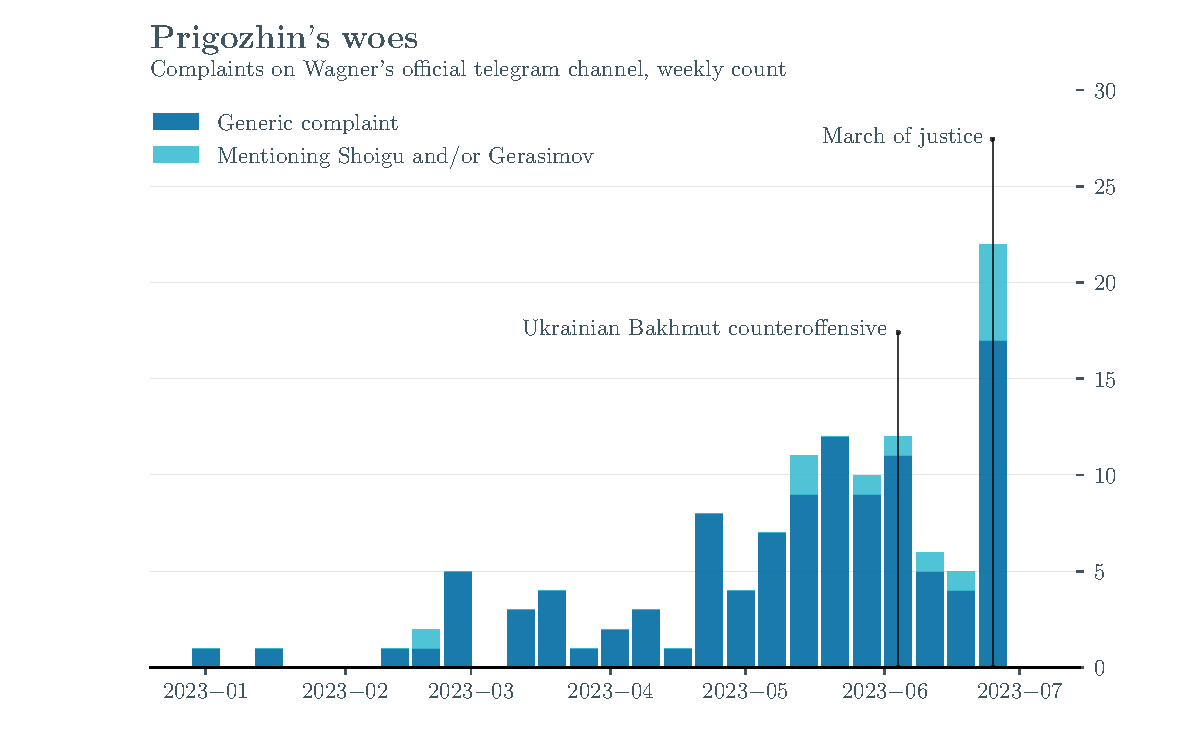
\includegraphics[height=8cm]{../../outputs/main_report/figures/hist.pdf}
\end{figure}

\vspace{0.5cm}
\noindent
Analyzing with AI over 400 audio files published from December 2022 to June 2023 allows to fully visualize the oligarch's growing boldness, escalating 
in constant complaints directly targeted at Russia's Minister of Difense Shoigu and Chief of General Staff Gerasimov after the Ukrainian counteroffensive in Bakhmut 
and in the lead-up to his armed rebellion.\\
Most of the messages mention Bakhmut and the surrounding villages, besieged and annexed by Wagner in May 2023 in what was Russia's only successful, albeit bloody, large 
scale offensive since the capture of Mariupol one year before. Rostov-on-Don, taken over by Wagner during the self-defined ``march of justice'' on 24 June 2023, is also mentioned several times. After the 
rebellion failed to reach its objectives silence fell over Wagner's Telegram channels, broken only by the news of Prigozhin's death in a plane crash exactly two months later. 

\begin{figure}[H]
    \centering
    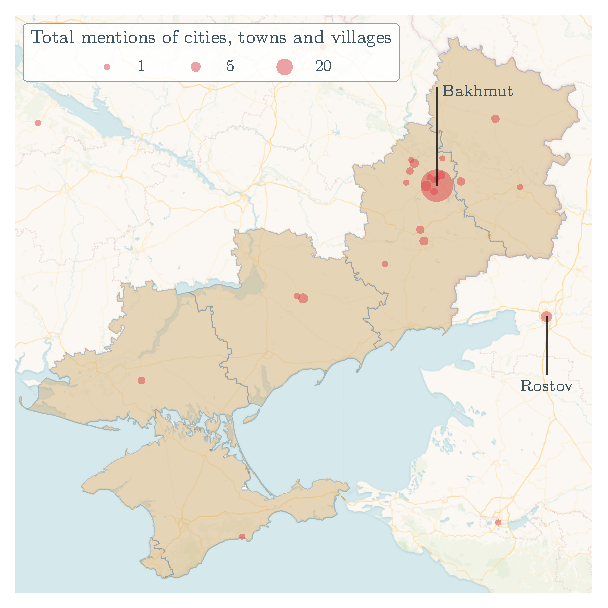
\includegraphics[height=8cm]{../../outputs/main_report/figures/map.pdf}
\end{figure}

\end{document}